\documentclass[a4paper, 11pt]{report}

\usepackage[utf8]{inputenc}
\usepackage[T1]{fontenc}
\usepackage[francais]{babel}
\usepackage{lmodern}
\usepackage[top = 2 cm, bottom = 2 cm, left = 2 cm, right = 2 cm]{geometry}
\usepackage{array}
\usepackage{graphicx}
\usepackage{color}
	\definecolor{orange}{RGB}{213, 107, 4}
\usepackage[colorlinks = true, urlcolor = orange]{hyperref}
\usepackage{caption}
\usepackage{fancyhdr}
\usepackage{verbatim}

\pagestyle{fancy}

\fancyhead[L]{Université Paris 13 Institut Galilée}

\title{Manuel d’utilisation de l’application GaliDAV}
\date{\today}

\begin{document}
	\makeatletter
	\begin{titlepage}
		\centering
		{\large \textsc{Université Paris 13}}\\
		{\large \textsc{École d’ingénieurs Sup Galilée}}\\
		\textsc{Spécialité Informatique 2\textsuperscript{e} année}\\
		\vspace{1cm}
		
\includegraphics[scale = 0.3]{logo_galilee.png}
		\hfill
		
\includegraphics[scale = 0.3]{logo_paris13.png}\\
		\vspace{1cm}
		\vfill
		{\LARGE \textbf{\@title}} \\
		\vspace{2em}
		{\large \@date} \\
		\vfill
		\hfill
	\end{titlepage}
	\makeatother
	\tableofcontents

	\chapter*{Avant-propos}
	\addcontentsline{toc}{chapter}{Avant-propos}
		GaliDAV a été initialement développé dans le cadre du cours de Conduite et gestion de projets à l’école d’ingénieurs SupGalilée de l’université Paris 13, par des étudiants en deuxième année de la spécialité informatique. Un dépôt sur GitHub est accessible à l’adresse : https://github.com/VeryTastyTomato/GaliDAV
	\chapter*{Introduction}
	\addcontentsline{toc}{chapter}{Introduction}
		\section*{Définition}
		\addcontentsline{toc}{section}{Définition}
			GaliDAV est une application web de gestion des emplois du temps. Elle est principalement développée en PHP. Elle permet d’élaborer et de gérer différents emplois du temps de plusieurs groupes d’individus, avec pour finalité la production d’un fichier PDF généré automatiquement et adapté aux individus auxquels il est destiné.
	\chapter{Installation}
		\section{Logiciels nécessaires}
			Avant d’installer GaliDAV, vous devez avoir installé et configuré les logiciels suivants :
			\begin{itemize}
				\item un serveur web (de préférence \href{http://httpd.apache.org/}{Apache HTTP Server}) ;
				\item \href{http://php.net/}{PHP}
				\item une base de données (de préférence \href{http://www.postgresql.org/}{PostgreSQL}) ;
				\item un serveur CalDAV (de préférence \href{http://www.davical.org/}{DAViCal}) ;
				\item et enfin le client CalDAV \href{http://agendav.org/}{AgenDAV}.
			\end{itemize}

			Nous allons indiquer par la suite une procédure d’installation de ces logiciels sous Debian (et qui devraient fonctionner pour ses dérivés).
		\section{Procédure d’installation sous Debian}
			Assurez-vous d’avoir installé les paquets suivants :
			\begin{itemize}
				\item \texttt{\textbf{apache2}} ;
				\item \texttt{\textbf{php5}}, \texttt{\textbf{php5-pgsql}}, \texttt{\textbf{php5-cli}} et \texttt{\textbf{php5-curl}} ;
				\item \texttt{\textbf{postgresql}} ;
				\item et enfin le paquet \texttt{\textbf{davical}}.
			\end{itemize}

			En ce qui concerne le client AgenDAV, vous devez télécharger l’archive contenant la version 1.2.6.2 sur son site officiel, la décompresser et copier le répertoire obtenu à l’emplacement \texttt{/usr/share/davical/htdocs} (nécessite les privilèges super-utilisateur). Il est fortement conseillé de renommer le répertoire décompressé \texttt{agendav}.

			Enfin, faites de même pour l’application GaliDAV, en veillant à ce que le répertoire soit nommé \texttt{galidav} (ce n’est pas obligatoire mais nous supposerons  que c’est le cas par la suite).
	\chapter{Configuration}
		\section{PostgreSQL}
			Après l’installation de PostgreSQL, il est fortement conseillé de changer le mot de passe de l’utilisateur \textit{postgres} en utilisant la commande suivant :
			\begin{verbatim}
				sudo passwd postgres
			\end{verbatim}

			Ensuite, ouvrez le fichier \texttt{/etc/postgresql/9.1/main/pg\_hba.conf} (toujours avec les privilèges super-utilisateur) et remplacer les \textit{trust} par \textit{md5}. Ensuite ajouter les lignes suivantes :
			\begin{verbatim}
				local   davical         davical_app                             trust
				local   davical         davical_dba                             trust
				local   agendav         agendav                                 trust
				local   galidav         galidav                                 trust
			\end{verbatim}

			\textbf{Remarque :} cette configuration n’est pas du tout sécurisée ; si vous souhaitez contrôler les connexions aux bases de données de manière sécurisée, consulter la documentation de PostgreSQL. De manière générale, la procédure décrite dans cette version du document ne prend en compte aucun problème de sécurité et n’est donc pas adapté pour des environnements en ayant besoin. \newline
			Ensuite, saisissez la commande suivante :
			\begin{verbatim}
				sudo -i -u postgres -c /usr/share/davical/dba/create-database.sh
			\end{verbatim}

			À ce stade, le mot de passe du compte administrateur de DAViCal s’affichera, notez-le soigneusement. Vous pourrez par la suite modifier le mot de passe du compte administrateur (fortement conseillé).
			Enfin, saisissez la commande suivante :
			\begin{verbatim}
				psql -U postgres
			\end{verbatim}

			et entrez ces requêtes :
			\begin{verbatim}
				CREATE USER agendav WITH PASSWORD 'votremotdepasse';
				CREATE DATABASE agendav ENCODING 'UTF8';
				GRANT ALL PRIVILEGES ON DATABASE agendav TO agendav;
				\q
			\end{verbatim}

		\section{Apache / DAViCal}
			Pour rendre le serveur DAViCal fonctionnel, on propose d’utiliser un hôte virtuel. Pour cela, vous devez tout d’abord connaître l’adresse IP de la machine sur laquelle se trouve le serveur DAViCal (qui peut-être différent de celle du serveur web). Ensuite, dans créez un fichier de configuration à l’emplacement \texttt{/etc/apache2/sites-available/} (nommez-le davical.conf par exemple) et saisissez dans ce fichier les lignes suivantes :
			\begin{verbatim}
				<VirtualHost *adresse ip*>
				  DocumentRoot /usr/share/davical/htdocs
				  DirectoryIndex index.php index.html
				  ServerName *nom de votre serveur*
				  ServerAlias *alias de votre serveur*
				  Alias /images/ /usr/share/davical/htdocs/images/
				  Alias /galidav /usr/share/davical/htdocs/galidav/web/public/
				  <Directory /usr/share/davical/htdocs/>
				      AllowOverride None
				      Order allow,deny
				      Allow from all
				  </Directory>
				  AcceptPathInfo On

				  php_value include_path /usr/share/awl/inc/
				  php_value include_path /usr/share/davical/inc/
				  php_value include_path /usr/share/davical/inc:/usr/share/awl/inc
				  # php_value magic_quotes_gpc 0
				  # php_value register_globals 0
				  php_value error_reporting "E_ALL & ~E_NOTICE"
				  # php_value default_charset "utf-8"
				</VirtualHost>
			\end{verbatim}

			Le texte entouré d’étoiles (*) est à remplacer par les valeurs correspondantes à votre cas. Les lignes commentées devant les php\_value le sont car elles ne devraient pas être nécessaires, mais s’il y a un souci réessayez en décommentant ces lignes.

			Modifier également le fichier également le fichier /etc/hosts en ajoutant une ligne contenant l’adresse IP indiqué dans l’hôte virtuel ci-dessus et le nom de domaine du serveur, indiqué aussi ci-dessus.

			Ensuite, utiliser la commande suivante :
			\begin{verbatim}
				sudo a2ensite davical.conf
			\end{verbatim}

			et recharger le serveur Apache :
			\begin{verbatim}
				sudo service apache2 reload
			\end{verbatim}

		\section{AgenDAV / GaliDAV}
			En supposant que l’on soit dans le répertoire \texttt{/etc/usr/share/davical/htdocs/galidav/}, saisissez la commande suivante :

			\begin{verbatim}
				psql -U agendav agendav < sql/pgsql.schema.sql
			\end{verbatim}
			Pour les autres paramètres, ils devraient normalement être correctement configurés, mais en cas de problème vous pouvez consulter la documentation d’AgenDAV ou contacter les développeurs de GaliDAV. En particulier, vous pouvez consulter la page suivante : \url{http://agendav.org/doc/1.2.6.2/admin/configuration.html}.

			En ce qui concerne GaliDAV, saisissez d’abord la commande suivante dans un terminal :
			\begin{verbatim}
				psql -U postgres
			\end{verbatim}

			puis entrez ces requêtes :
			\begin{verbatim}
				CREATE USER galidav;
				CREATE DATABASE galidav ENCODING 'UTF8';
				GRANT ALL PRIVILEGES ON DATABASE galidav TO galidav;
				\q
			\end{verbatim}
		\section{Documentations externes}
			En cas de difficultés, ces sites web peuvent contenir des informations susceptibles de vous aider :
			\begin{itemize}
				\item \url{http://doc.ubuntu-fr.org/postgresql} ;
				\item \url{http://postgresql.fr/guidedemarragerapide} ;
				\item \url{http://doc.ubuntu-fr.org/davical} ;
				\item \url{http://davical.org/installation.php} ;
				\item \url{http://doc.ubuntu-fr.org/tutoriel/virtualhosts_avec_apache2} ;
				\item \url{http://agendav.org/doc/1.2.6.2/}.
			\end{itemize}

	\chapter{Utilisation}
		Dans l’application GaliDAV, chaque matière est représentée par un \emph{calendrier} , et un cours (cours magistral, travaux dirigés, travaux pratiques, etc.) est représenté par un \emph{événement}.
		\section{Ajouter une matière}
			Afin d’ajouter une matière, il suffit d’ajouter un calendrier dans le panneau des calendriers à gauche. Une boîte de dialogue va alors s’ouvrir, vous demandant de saisir le nom de ce calendrier et de choisir sa couleur.

			\begin{center}
				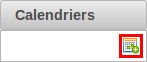
\includegraphics[scale = 1]{ajouter_calendrier.png}
				\captionof{figure}{Bouton permettant d’ajouter un calendrier (donc une matière)}
			\end{center}
		\section{Modifier une matière}
			Vous pouvez par la suite modifier ce calendrier en cliquant sur les engrenages qui apparaissent lorsque votre curseur le survole dans le panneau des calendriers. Une boîte de dialogue s’ouvrira alors. Dans l’onglet \textbf{Options générales}, vous pouvez modifier le nom et la couleur du calendrier. Il vous suffit ensuite de cliquer sur le bouton \textbf{Enregistrer} pour valider les modifications.

			\begin{center}
				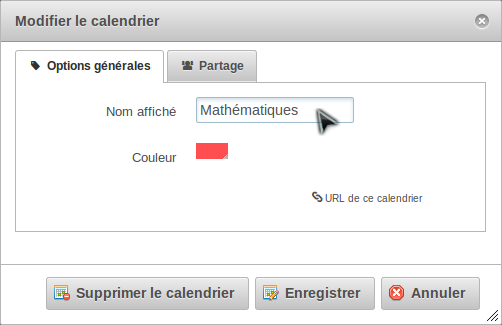
\includegraphics[scale = 0.7]{modifier_calendrier.png}
				\captionof{figure}{Boîte de dialogue permettant de modifier un calendrier (donc une matière)}
			\end{center}

		\section{\og Partager \fg{} une matière}
			\begin{center}
				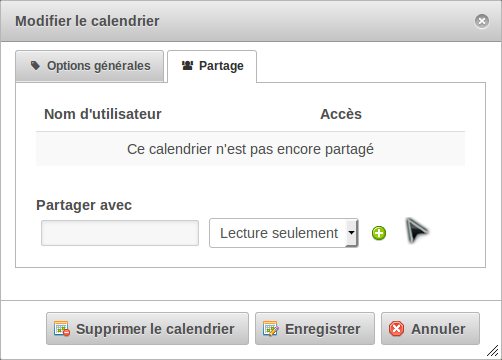
\includegraphics[scale = 0.7]{partager_calendrier.png}
				\captionof{figure}{Partage d’un calendrier (donc d’une matière)}
			\end{center}

			La figure 3.2 montre la boîte de dialogue permettant de partager un calendrier. On y accède en cliquant sur les engrenages dans le panneau des calendriers, puis en cliquant sur l’onglet \textbf{Partage}. Il suffit d’écrire l’identifiant de la personne avec qui partager le calendrier, ainsi que de sélectionner le mode de partage. Deux modes sont disponibles : partage en \textit{Lecture seulement} et partage en \textit{Lecture et écriture}. Une fois cela fait, cliquer sur le bouton + en vert. N’oubliez pas de cliquer sur le bouton \textbf{Enregister} pour valider les modifications, ou cliquer sur le bouton \textbf{Annuler} si vous ne voulez pas appliquer les modifications.

			Lorsqu’un calendrier est partagé par un utilisateur vers un autre, celui qui est le destinataire du partage voit apparaître dans son interface un nouveau panneau intitulé \textbf{Calendriers partagés}. En cliquant sur le petit œil barré en bas à droite de ce panneau, il peut masquer tous les calendriers partagés.

			Quand à celui qui a partagé son calendrier, un symbole d’une flèche sortant d’un cadre apparaît à gauche de ces calendriers dans le panneau des calendriers.

			\begin{center}
				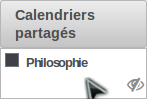
\includegraphics[scale = 1]{calendriers_partages.png}
				\captionof{figure}{Panneau des calendriers partagés}
			\end{center}

		\section{Supprimer une matière}
			Après avoir cliqué sur les engrenages d’un calendrier dans le panneau de gauche, cliquer sur le bouton \textbf{Supprimer le calendrier} dans la boîte de dialogue.

		\section{Ajouter un cours, un TD, un TP…}
			Pour ajouter un cours (ou un TD, un TP, etc.) d’une matière (correspondant à un calendrier), il suffit de cliquer sur \textbf{Créer un événement} à gauche. Vous pouvez également directement cliquer sur le panneau principal, vous pourrez ainsi régler la date et les heures de début et de fin de l’événement directement. Une boîte de dialogue surgira ensuite, vous demandant de multiples informations dans l’onglet \textbf{Options générales}.

			Dans le champ \textbf{Résumé}, saisissez les informations que vous souhaitez afficher, typiquement le type de cours (cours magistral, TP, TP…) et la salle. Dans le champ \textbf{Calendrier}, sélectionner dans la liste déroulante la matière du cours que vous souhaitez ajouter. Le calendrier sélectionné par défaut peut-être modifié dans vos préférences, voir la section concernée. Les champs \textbf{Date de début} et \textbf{Date de fin} permettent de sélectionner les jours et heures de début et de fin d’un événement.

			Dans l’onglet \textbf{Répétitions}, vous pouvez régler la fréquence de répétitions (champ \textbf{Répétition}) de l’événement. Vous pouvez ensuite régler le nombre d’occurrences de cet événement (champ \textbf{Nombre de répétitions}) ou la date de fin de la récurrence de l’événement (champ \textbf{Jusqu’à}) (mais pas les deux en même temps). Vous pouvez à ce stade cliquer sur \textbf{Enregistrer} pour effectivement créer l’événement ou cliquer sur \textbf{Annuler} si vous ne souhaitez plus le créer.

			\begin{center}
				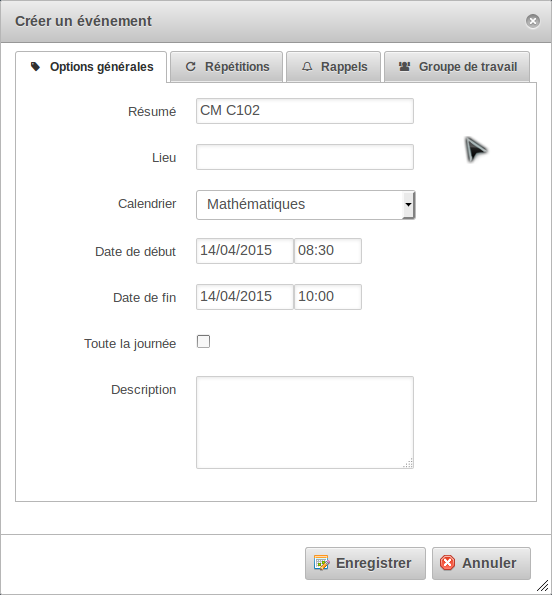
\includegraphics[scale = 0.7]{creer_evenement.png}
				\captionof{figure}{Créer un évènement (donc un cours, TD, TP…)}
			\end{center}
		\section{Modifier un cours, un TD, un TP…}
			Pour modifier un cours (ou un TD, un TP, etc.) existant, il suffit de cliquer sur l’événement le représentant dans le panneau principal, puis de cliquer sur le bouton \textbf{Modifier}. Vous pouvez également glisser-déposer un événement dans le panneau principal pour modifier sa date ainsi que son heure de début et de fin. Vous pouvez également modifier sa durée en cliquant sur sa double barre horizontale puis en tirant vers le haut ou vers le bas selon que vous souhaitez diminuer ou augmenter sa durée. Veuillez noter que ces deux dernières opérations ne sont pas disponibles pour les événements récurrents (qui sont indiqués par une petite flèche bouclée).

			\begin{center}
				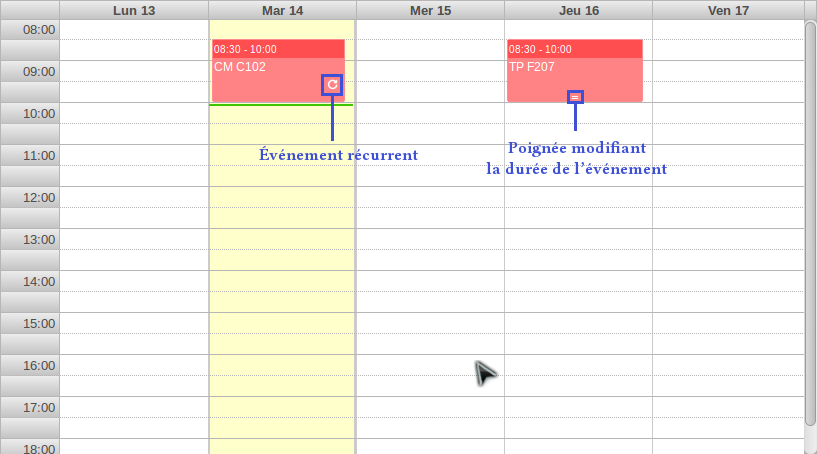
\includegraphics[scale = 0.6]{modifier_evenement.png}
				\captionof{figure}{Les deux types d’événements}
			\end{center}
		\section{Supprimer un cours, un TD, un TP…}
			Il suffit pour cela de cliquer sur l’événement dans le panneau principal puis de cliquer sur le bouton \textbf{Supprimer}. Une boîte de dialogue demandant une confirmation s’affichera, cliquer alors sur le bouton \textbf{Oui}.

		\section{Modifier l’affichage}
			Vous pouvez modifier la plage d’affichage du calendrier du panneau principal. Il y a 3 vues différentes : \textbf{mois}, \textbf{semaine} et \textbf{jour}. Ces boutons se trouvent au-dessus du calendrier du panneau principal.

			\begin{center}
				
\includegraphics[scale = 1]{afficher_differentes_vues}
				\captionof{figure}{Boutons permettant de modifier l’affichage du calendrier}
			\end{center}
		\section{Naviguer dans le calendrier}
			Les boutons de la figure permettent de naviguer dans le calendrier. Selon la vue actuellement affichée, les flèches permettent de se déplacer de jour en jour, de semaine en semaine ou de mois en mois. Le bouton \textbf{Aujourd’hui} permet évidemment de revenir immédiatement au jour, semaine ou mois actuel. Si vous souhaitez vous rendre à une date particulière, cliquer sur bouton ayant une icône d’agenda ; un petit calendrier surgira, vous permettant de naviguer et de sélectionner la date à laquelle vous souhaitez vous rendre.

			\begin{center}
				
\includegraphics[scale = 1]{naviguer_dans_calendrier.png}
				\captionof{figure}{Boutons permettant de naviguer dans le calendrier}
			\end{center}
		\section{Préférences}
			Pour accéder au menu des préférences, cliquer votre identifiant et sélectionner \textbf{Préférences}. Vous pouvez régler le calendrier dans lequel les événements seront ajoutés par défaut. Vous pouvez également choisir de masquer des calendriers.

			\begin{center}
				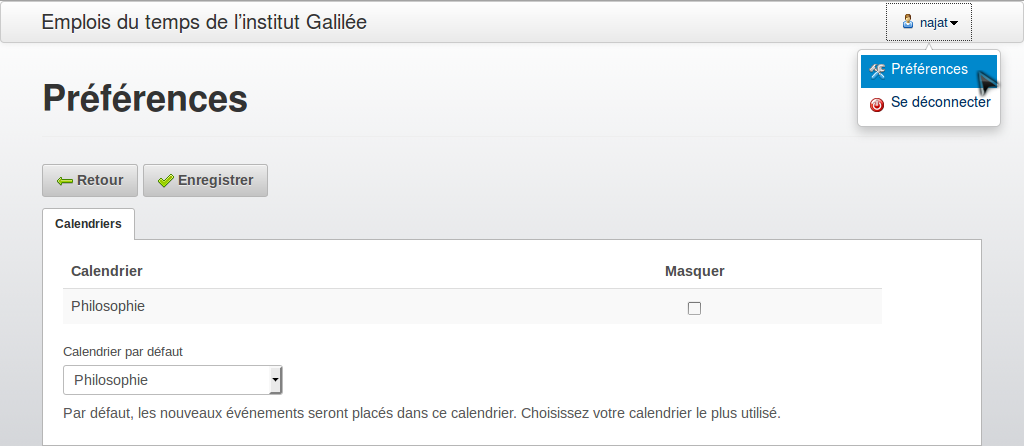
\includegraphics[scale = 0.45]{preferences.png}
				\captionof{figure}{Page des préférences}
			\end{center}
\end{document}